\documentclass{beamer}

\usetheme{Amsterdam}

\usepackage{caption}

\begin{document}
\title{Parameter Inference with Gravitational Wave and Electromagnetic Data}
\subtitle{RIT Undergraduate Research Symposium}
\author{Ben Champion}
\institute{Rochester Institute of Technology \\ Center for Computational Relativity and Gravitation}

% logos
\titlegraphic{
\includegraphics[width=6cm]{Images/RIT_RGB_hor_k}\hspace*{2cm}~%
   
\includegraphics[width=2cm]{Images/ccrg_logo}
}

\date{
  August 1, 2019
}

\frame{
  \titlepage
}

\frame{ \frametitle{Table of contents}
  \tableofcontents
}

\section{GW Parameter Estimation}

\frame{ \frametitle{Gravitational Wave Astrophysics}
  \begin{itemize}
    \item Objects with mass cause distortions in spacetime \pause
    \item Motion involving a changing acceleration produces gravitational waves \pause
    \begin{itemize}
      \item (assuming this motion does not involve spherical or rotational symmetry) \pause
    \end{itemize}
    \item The gravitational waves produced by most objects are too small to detect \pause
    \item Gravitational waves produced by merging black holes or neutron stars are large enough to detect
  \end{itemize}
}

\frame{ \frametitle{Gravitational Wave Parameter Estimation}
  \begin{itemize}
    \item Estimation of astrophysical source parameters from observations \pause
    \begin{itemize}
      \item Intrinsic parameters: \pause
      \begin{itemize}
        \item Mass \pause
        \item Spin \pause
      \end{itemize}
      \item Extrinsic parameters: \pause
      \begin{itemize}
        \item Sky location \pause
        \item Distance \pause
        \item Orientation \pause
      \end{itemize}
    \end{itemize}
  \item Goal is to recover a \textit{posterior distribution} of parameters, using theoretical models that give waveforms as functions of these parameters
  \end{itemize}
}

\frame{ \frametitle{Bayes' Theorem and Model Likelihoods}
  For a vector of unknown parameters $\vec \theta$, proposed waveform model $H$, and set of observations $\{d\}$, Bayes' Theorem gives the \textit{probability density function} of $\vec \theta$ as
  \begin{align*}
    p(\vec \theta | \{d\}, H) = \frac {p(\vec \theta | H) p(\{d\} | \vec \theta, H)} {P(\{d\} | H)}
  \end{align*} \pause
  \begin{itemize}
    \item $p(\vec \theta | H)$ is the \textit{prior} distribution of $\vec \theta$ \pause
    \item $p(\{d\} | \vec \theta, H)$ is the \textit{likelihood function} - the likelihood of observing $\{d\}$ given $\vec \theta$ and $H$ \pause
    \begin{itemize}
      \item Function of residuals - differences between model and data \pause
    \end{itemize}
    \item $P(\{d\} | H)$ is called the \textit{evidence} for a model (a constant for each model)
  \end{itemize}
}

\frame{ \frametitle{Posterior Distribution}
  \begin{columns}
      \column{2.0in}
      \begin{itemize}
          \item To plot the posterior distribution of the parameters: \pause
          \begin{itemize}
              \item Sample the parameter space \pause
              \item Calculate the probability of each sampled point \pause 
          \end{itemize}
      \end{itemize}
      \column{3.0in}
      \begin{figure}
        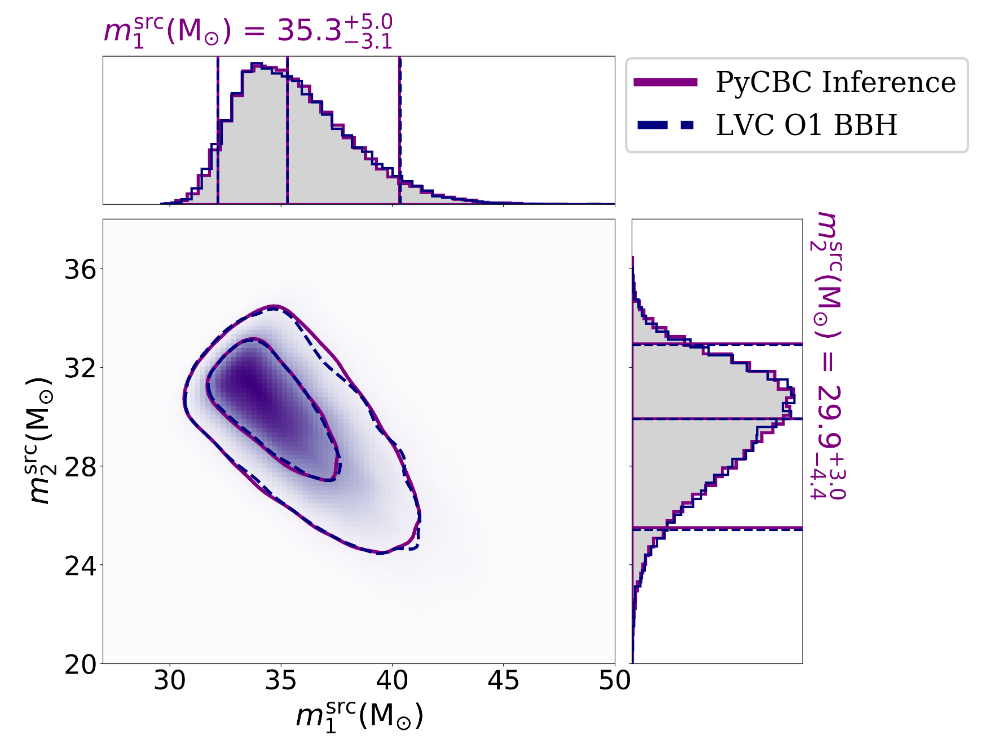
\includegraphics[width=2.5in]{Images/corner_example}
        \caption*{Example of posterior distribution of masses for GW150914 (arXiv:1807.10312)}
      \end{figure}
  \end{columns}
}

\section{Multimessenger Parameter Estimation}

\frame{ \frametitle{Neutron Star Mergers and Kilonovae}
    \begin{itemize}
      \item Binary neutron star (BNS) mergers produce gravitational waves \pause
      \item Kilonovae - supernova-like explosions resulting from BNS mergers - are a primary candidate for the creation of heavy elements (such as gold) in the universe \pause
      \item Kilonovae eject large amounts of material at high velocities \pause
      \item They produce electromagnetic (EM) transients through the radioactive decay of this ejected material \pause
      \item These EM signals can be observed and used in the analysis of BNS mergers \pause
      \item GW170817: first BNS merger detected by LIGO, accompanied by electromagnetic observations across frequency bands
    \end{itemize}
}

\frame{ \frametitle{Multimessenger Astrophysics}
    \begin{figure}
      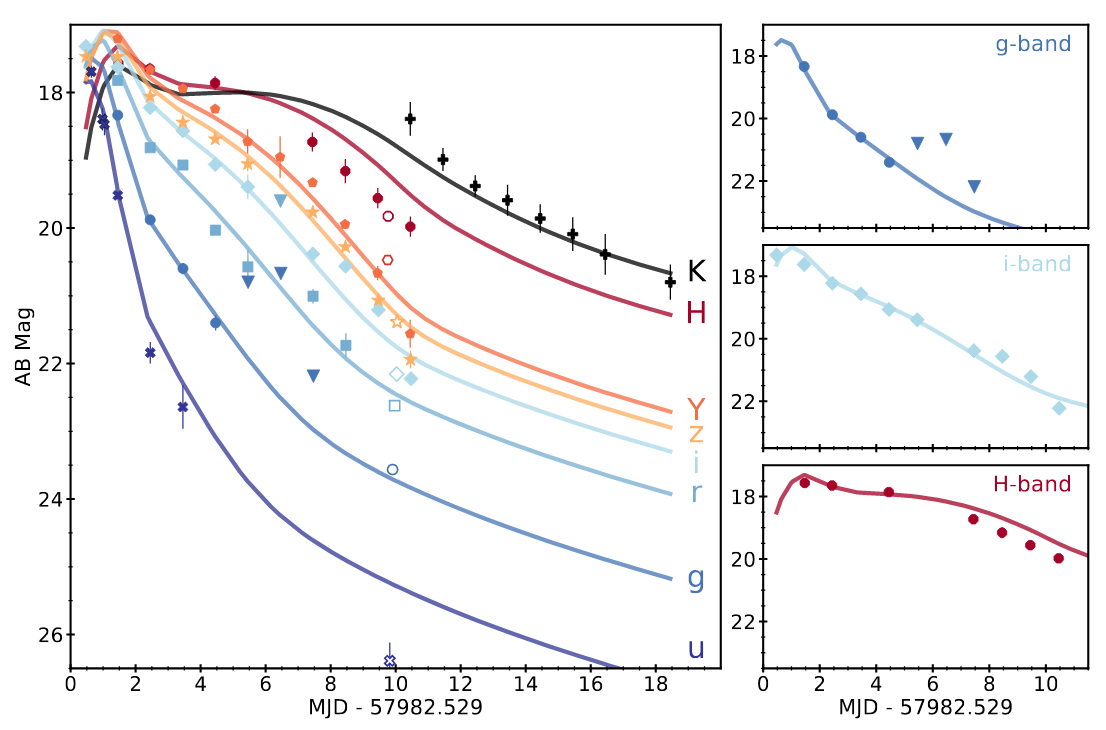
\includegraphics[width=3.0in]{Images/lightcurves}
      \caption*{GW170817 lightcurves (arXiv:1710.05840)}
    \end{figure}
    Lightcurve: light intensity as a function of time
}

\frame{ \frametitle{Multimessenger Astrophysics}
    \begin{figure}
      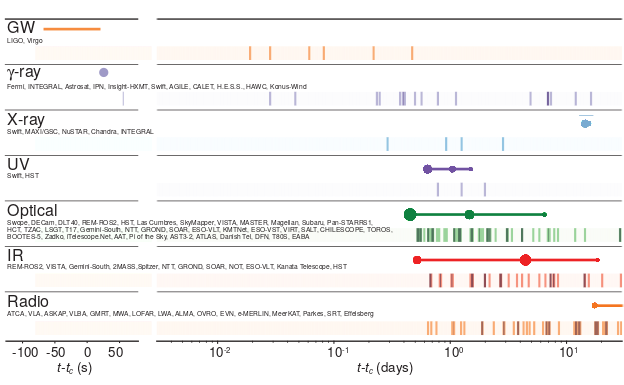
\includegraphics[width=4.0in]{Images/timeline}
      \caption*{GW170817 timeline of detections (arXiv:1710.05833)}
    \end{figure}
}

\frame{ \frametitle{EM Parameter Estimation}
  \begin{itemize}
    \item Parameter estimation using EM data channels is similar to gravitational wave parameter estimation \pause
    \item Likelihood function used for EM parameter estimation: the log-likelihood of parameter vector $\vec \theta$ is
    \begin{align*}
      \ln L = -0.5 \sum \frac {(x(t) - m(t | \vec \theta))^2} {\Delta x(t)^2 + \Delta m(t | \vec \theta)^2}
    \end{align*} \pause
    where $x(t)$ is the lightcurve magnitude at time $t$, $m(t | \vec \theta)$ is the model value at time $t$ given the current model parameters, $\Delta x(t)$ is the data error, and $\Delta m(t | \vec \theta)$ is the model error.
  \end{itemize}
}

\begin{frame}[fragile] \frametitle{\texttt{EM\_PE}: Rapid Parameter Estimation for EM Transients}
    \begin{itemize}
      \item Open-source \texttt{Python} package: \texttt{github.com/bwc3252/EM\_PE} \pause
      \item Parameter estimation for arbitrary models and data channels \pause
      \item Uses adaptive Monte Carlo integration to sample parameter space \pause
      \item Functionality: \pause
      \begin{itemize}
        \item Full PE \pause
        \item Visualization of results \pause
        \item Likelihood function for use in other PE codes
      \end{itemize}
    \end{itemize}
\end{frame}

\frame{ \frametitle{Multimessenger PE}
    \begin{itemize}
        \item GW and EM data can be used together \pause
        \begin{itemize}
            \item $lnL = lnL_{GW} + lnL_{EM}$ \pause
        \end{itemize}
        \item The likelihood function provided by the \texttt{EM\_PE} package can be imported and used in existing GW codes
    \end{itemize}
}

\frame{ \frametitle{Results}
}

\end{document}
